In this problem, the following linearized Korteweg-deVries (KdV) equation is considered on the interval $x \in [-1, 1], \hspace{1mm} t > 0, $

\begin{equation}
\label{KdV}
    u_t + (1+\pi^2)u_x + u_{xxx} = 0, \hspace{1mm} u(x,0) = \sin{(\pi x)}.
\end{equation}
A periodic boundary condition with period 2, i.e. $u(x+2, t) = u(x,t)$, is assumed. Hence, the function may be studied only on the interval $[-1, 1]$. The grid points

\begin{equation*}
    x_0 = -1, \, x_1 = -1 + \frac{2}{M}, \, \dots, \, x_M = 1,
\end{equation*}
are considered.

\subsubsection{a)}
In order to solve equation \eqref{KdV} numerically, it has to be discretized in time and space. Let $u_m^n := u(x_m,t_n)$ where $x_m=-1+mh \text{,  } 0 \leq m \leq M$ and $h=\frac{2}{M}$. The central difference approximation for the first derivative defined in \eqref{Theory_approx_first_derivative} in section \ref{section_2.2} is used to approximate the first spatial derivative. Thus, the approximation of $(u')_m:=u_x(x_m)$ at time step $t=t_n$ is

\begin{equation}
\begin{split}
\label{task4firstdisc}
 (u')_m &= \frac{1}{h} \mu \delta_x u_m + \mathcal{O}(h^2) \\ &= \frac{1}{2h} \left(u_{m+1} - u_{m-1}\right) + \mathcal{O}(h^2).
\end{split}
\end{equation}
Similarly, a discrete approximation for the third derivative $(u''')_m:=u_{xxx}(x_m)$ at $t=t_n$ is

\begin{equation}
\begin{split}
\label{task4thirdisc}
 (u''')_m &= \frac{1}{h^3} (\mu \delta_x)^3 u_m + \mathcal{O}(h^2) = \frac{1}{2h^3} (\mu \delta_x)^2 \left(u_{m+1}-u_{m-1}\right) + \mathcal{O}(h^2) \\ &= \frac{1}{4h^3} \mu \delta_x \left(u_{m+2}-2u_m + u_{m-2}\right) + \mathcal{O}(h^2) \\ &= \frac{1}{8h^3} \left(u_{m+3}-3u_{m+1}+3u_{m-1}-u_{m-3}\right) + \mathcal{O}(h^2). 
\end{split}
\end{equation}
Both these discretizations have a local truncation error of $\mathcal{O}(h^2)$. For the discretization in the temporal direction, both Euler's method and the Crank-Nicolson (trapezoidal) method are used. \newline

The temporal discretization using Euler's method can be derived as follows. The step size in the temporal direction is denoted by $k$. An expansion of the exact solution $u_m^{n+1}$ for constant $x = x_m$ around $t = t_n$ yields 

\begin{equation*}
\begin{split}
    u_m^{n+1} &= u_m^n + k \partial_tu_m^n + \frac12k^2\partial^2_tu_m^n + \dots \\ 
    &= u_m^n - k((1+\pi^2)(u')_m + (u''')_m) + \mathcal{O}(k^2), 
\end{split}
\end{equation*}
where equation \eqref{KdV} has been used in the second equality. Now, inserting the two spacial discretizations \eqref{task4firstdisc} and \eqref{task4thirdisc} gives

\begin{equation}
\begin{split}
\label{task4EulerExact}
    u_m^{n+1} &= u_m^n - k((1+\pi^2)(u')_m + (u''')_m) + \mathcal{O}(k^2)\\ 
    &= u_m^n - k\left(\frac{1+\pi^2}{2h}(u_{m+1}^n - u_{m-1}^n) + \frac{1}{8h^3}(u_{m+3}^n - 3u_{m+1}^n + 3u_{m-1}^n - u_{m-3}^n)\right) \\& \hspace{10mm} + \mathcal{O}(k^2 + kh^2)\\
    &= u_m^n - \frac{k}{2h}\left(\frac{1}{4h^2}u_{m+3}^n+\left[1+\pi^2 - \frac{3}{4h^2}\right]u_{m+1}^n-\left[1+\pi^2 - \frac{3}{4h^2}\right]u_{m-1}^n-\frac{1}{4h^2}u_{m-3}^n\right) \\& \hspace{10mm} + \mathcal{O}(k^2 + k h^2),
\end{split}
\end{equation}
which has a truncation error, $\tau_m^n$, of order $\mathcal{O}(k + h^2)$, since $k\tau_m^n = \mathcal{O}(k^2 + kh^2)$. The notation $U_m^n$ is adopted to specify the approximate solution of $u_m^n$, i.e. in the point $(x_m, t_n)$. Inserting this approximate solution into the equation \eqref{task4EulerExact} and neglecting the truncation error yields the difference scheme 

\begin{equation}
\label{task4discEuler}
    U_m^{n+1} = U_m^n + k\left(-aU_{m+3}^n-b U_{m+1}^n+bU_{m-1}^n+aU_{m-3}^n\right),
\end{equation}
where the coefficients $a$ and $b$ are defined as

\begin{equation}
\label{constants_spatialdiscretization}
    a = \frac{1}{8h^3} \text{,} \hspace{4mm}
    b = \frac{1+\pi^2}{2h} - \frac{3}{8h^3}.
\end{equation}
\newline

Crank-Nicolson is based on the trapezoidal rule, which gives a slightly different derivation of the temporal discretization when using this method. The fundamental theorem of calculus, together with the trapezoidal quadrature, yield

\begin{equation*}
\begin{split}
    u(x_m, t_{n+1}) - u(x_m, t_n) & = \int_{t_n}^{t_{n+1}} u_t(x_m, t)\mathrm{d}t \\
    &= \frac{t_{n+1}-t_n}{2} \left(u_t(x_m,t_{n+1}) + u_t(x_m,t_n))\right) + \mathcal{O}((t_{n+1}-t_n)^3) \\
    &= \frac{1}{2}k \left(u_t(x_m,t_{n+1})+u_t(x_m,t_n))\right) + \mathcal{O}(k^3).
\end{split}
\end{equation*}
This expression, together with the (KdV)-equation \eqref{KdV}, leads to 

\begin{equation}
\begin{split}
    u_m^{n+1} &= u_m^n + \frac12k(\partial_tu_m^n + \partial_tu_m^{n+1}) + \mathcal{O}(k^3) \\
    &= u_m^n - \frac12k((1+\pi^2)(u')_m^{n} + (u''')_m^{n}+(1+\pi^2)(u')_m^{n+1} + (u''')_m^{n+1}) + \mathcal{O}(k^3) \\
    &= u_m^n - \frac12k((1+\pi^2)((u')_m^{n} + (u')_m^{n+1}) + (u''')_m^{n} + (u''')_m^{n+1}) + \mathcal{O}(k^3), 
\end{split}
\end{equation}
where the $\mathcal{O}(k^3)$-error stems from the trapezoidal quadrature. Also, a superscript $n$ or $n+1$ is added to the derivative approximations, to signal at which point in time the functions are evaluated. Inserting the two spacial discretizations \eqref{task4firstdisc} and \eqref{task4thirdisc} yields

\begin{equation}
\begin{split}
\label{task4CrankExact}
    u_m^{n+1} &= u_m^n - \frac12k((1+\pi^2)((u')_m^{n} + (u')_m^{n+1}) + (u''')_m^{n} + (u''')_m^{n+1}) + \mathcal{O}(k^3) \\
    &= u_m^n - \frac12k\left(\frac{1+\pi^2}{2h}(u_{m+1}^n - u_{m-1}^n + u_{m+1}^{n+1} - u_{m-1}^{n+1}) \right.\\ &\left.+ \frac{1}{8h^3}(u_{m+3}^n - 3u_{m+1}^n + 3u_{m-1}^n - u_{m-3}^n + u_{m+3}^{n+1} - 3u_{m+1}^{n+1} + 3u_{m-1}^{n+1} - u_{m-3}^{n+1})\right) + \mathcal{O}(k^3 + k h^2)\\
    &= u_m^n + \frac{k}{2}\left( \frac{1}{8h^3}(-u_{m+3}^{n+1} + u_{m-3}^{n+1}-u_{m+3}^n + u_{m-3}^n) \right.\\ &\left.+ \left(\frac{1+\pi^2}{2h}-\frac{3}{8h^3}\right) (-u_{m+1}^{n+1} + u_{m-1}^{n+1}-u_{m+1}^n+u_{m-1}^n) \right) + \mathcal{O}(k^3 + k h^2).
\end{split}
\end{equation}
Finally, insertion of the approximate solution $U$ into the equation \eqref{task4CrankExact}, while neglecting the truncation error, and making use of the coefficients defined in \eqref{constants_spatialdiscretization}, gives the difference scheme 

\begin{equation}
\begin{split}
\label{task4discCrank}
    U_m^{n+1} = U_m^n + \frac{k}{2}\left(-a U_{m+3}^{n+1} - b U_{m+1}^{n+1} + b U_{m-1}^{n+1} + a U_{m-3}^{n+1} - a U_{m+3}^n - b U_{m+1}^n + b U_{m-1}^n +a U_{m-3}^n \right).
\end{split}
\end{equation}

\subsubsection*{Von Neumann stability}
Next in line is to examine if these two discretization methods are Von Neumann stable. The discretization based on Euler's method \eqref{task4discEuler} is examined first. Assume solutions of the form $U_m^n = \xi^n \mathrm{e}^{i\beta x_m}$ with $x_m = -1 + mh$. Insertion into the discretization formula yields an equation where all the terms contain the expression $\mathrm{e}^{-i\beta}$. Dividing the equation by this exponential expression yields 

\begin{equation*}
    \xi^{n+1} \mathrm{e}^{i\beta mh} = \xi^n \mathrm{e}^{i\beta mh} + k\xi^n (-a \mathrm{e}^{i\beta (m+3)h} - b\mathrm{e}^{i\beta (m+1)h} +b\mathrm{e}^{i\beta (m-1)h} +a \mathrm{e}^{i\beta (m-3)h}).
\end{equation*}
Moreover, dividing the equation by $\xi^n \mathrm{e}^{i\beta m h}$ leads to 

\begin{equation*}
\begin{split}
    \xi &= 1 + k(-a \mathrm{e}^{3 i\beta h} - b \mathrm{e}^{i\beta h} + b\mathrm{e}^{-i\beta h} + a\mathrm{e}^{-3 i\beta h}) \\
    &= 1 - 2ki(a \sin{(3 \beta h)} + b \sin{(\beta h)}).\\
\end{split}
\end{equation*}
Now, using the fact that $\sin{(3x)} = 3\sin{(x)} - 4\sin^3{(x)}$ and that $b = \frac{1+\pi^2}{2h} - 3a$, yields

\begin{align}
    \xi &= 1 - 2ki\left(3a\sin{(\beta h)}-4a\sin^3{(\beta h)}+\left(\frac{1+\pi^2}{2h}-3a\right)\sin{(\beta h)}\right) \nonumber\\
    &= 1 -2ki\left(\left(\frac{1+\pi^2}{2h}\right)\sin{(\beta h)}-4a\sin^3{(\beta h)}\right)\nonumber \\
    &= 1 + i\frac{k}{h}\sin{(\beta h)} \left(\frac{\sin^2{(\beta h)}}{h^2}-(1+\pi^2)\right),
    \label{xiEulerTask4a}
\end{align}
where $a=\frac{1}{8h^3}$ has been inserted in the last step. To achieve Von Neumann stability, the condition $|\xi| \leq 1 + \mu k$, where $\mu \geq 0$ is a constant independent of $h$ and $k$, needs to be satisfied. The Von Neumann stability criterion is equivalently stated as 

\begin{equation*}
    |\xi|^2 \leq 1 + 2\mu k + (\mu k)^2.
\end{equation*}
The squared modulus of equation \eqref{xiEulerTask4a} is given as
\begin{align*}
    |\xi|^2 &= 1 + \frac{k^2}{h^2}\sin^2{(\beta h)} \left(\frac{\sin^2{(\beta h)}}{h^2}-(1+\pi^2)\right)^2 \nonumber \\ &= 1 + k^2 \beta_h^2 \left(\beta_h^2 - C^2\right)^2,
    %\label{xi^2Euler}
\end{align*}
where the quantities $C:=\sqrt{1+¨\pi^2}$ and $\beta_h:=\frac{\sin{(\beta h)}}{h}$ are defined. Assuming (by contradiction) that the Von Neumann criterion is satisfied gives

\begin{equation*}
    \begin{split}
        & 2\mu k + \mu^2 k^2 -k^2 \beta_h^2 \left(\beta_h^2 - C^2\right)^2 \geq 0\\ & \Rightarrow \mu^2 k^2 + 2\mu k - k^2 \beta_h^2\left(\beta_h^2 -C^2\right)^2 = D \text{,} \hspace{2mm} D \geq 0 \\ \text{(abc-formula) }&\Rightarrow \mu = \frac{1}{k} \left(-1 \pm \sqrt{1 + D + k^2 \beta_h^2 (\beta_h^2-C^2)^2}\right).
    \end{split}
\end{equation*}
Observe that it is possible for $\mu$ to be a non-negative constant if the positive solution of the quadratic formula is chosen. Furthermore, independence of $\mu$ from $h$ and $k$ is only possible if $\mu=0$. These observations yield

\begin{equation*}
    \begin{split}
        &\mu = 0 \Rightarrow -1 + \sqrt{1 + D + k^2 \beta_h^2 (\beta_h^2-C^2)^2} = 0 \\ & \Rightarrow D = -k^2 \beta_h^2(\beta_h^2-C^2)^2.
    \end{split}
\end{equation*}
The last equation is clearly a contradiction to the criterion that $D \geq 0$. Hence, there exists no positive constant $\mu$ independent of $h$ and $k$ that satisfies the Von Neumann criterion. Conclusively, the discretization based on Euler's method \eqref{task4discEuler} is not Von Neumann stable. 
\begin{comment}
\textcolor{red}{The old version;}
For Euler's method, such a constant $\mu$ does not exist, because

\begin{align}
    |\xi|^2 &= 1 + \frac{k^2}{h^2}\sin^2{(\beta h)} \left(\frac{\sin^2{(\beta h)}}{h^2}-(1+\pi^2)\right)^2 \nonumber \\
    &= 1 + \frac{k^2}{h^2}\sin^2{(\beta h)}\left(\frac{\sin^4{(\beta h)}}{h^4} - 2\frac{\sin^2{(\beta h)}}{h^2}(1+\pi^2) + (1+\pi^2)^2\right) \nonumber \\
    &= 1 + \frac{k^2}{h^2}\sin^2{(\beta h)}\left(\frac{\sin^4{(\beta h)}}{h^4} - 2\frac{\sin^2{(\beta h)}}{h^2}C + C^2\right),
    \label{xi^2Euler}
\end{align}
where the constant value $C = (1+\pi^2)$ is highlighted by redefinition. It is apparent that it is impossible to bound \eqref{xi^2Euler} by $1 + 2\mu k + (\mu k)^2$, since a constant $\mu \geq 0$ independent of $h$ and $k$ is not possible to define. In fact, asymptotically, the expression \eqref{xi^2Euler}  is bounded by $u = 1 + \mathcal{O}(h^{-6})$, where $u \overset{h \rightarrow 0} \longrightarrow \infty$. The forward Euler method \eqref{task4discEuler} is therefore not Von Neumann stable.\textcolor{red}{stop old version.} \newline
\end{comment}

Next, the discretization based on Crank-Nicolson \eqref{task4discCrank}, is examined. In a similar manner, it is assumed that $U_m^n = \xi^n \mathrm{e}^{i\beta x_m}$ and $x_m = -1 + mh$. Insertion into the discretization formula and dividing the equation by $\xi^n \mathrm{e}^{i \beta m h}\mathrm{e}^{-i\beta}$ yields

\begin{equation*}
\begin{split}
    \xi  &= 1+ \frac{k}{2} \left(-a\xi \mathrm{e}^{3i \beta h} -b\xi \mathrm{e}^{i \beta h} + b\xi \mathrm{e}^{-i \beta h}+a\xi \mathrm{e}^{-3 i \beta h} - a\mathrm{e}^{3i \beta h}-b\mathrm{e}^{i \beta h}+b\mathrm{e}^{-i \beta h}+a\mathrm{e}^{-3i \beta h}\right)\\
    &= 1 -k i\left(a\xi \sin{(3 \beta h)} +b\xi \sin{(\beta h)} + a\sin{(3\beta h)}+b\sin{(\beta h)} \right)\\ \vspace{2mm}
    &\Rightarrow \xi + k i \xi \left(a \sin{(3\beta h)}+b\sin{(\beta h)}\right) = 1 - ki\left(a\sin{(3\beta h)+b\sin{(\beta h)}} \right)\\
    &\Rightarrow \xi = \frac{1 -ki\left(a \sin{(3\beta h)}+b\sin{(\beta h)}\right)}{1+ki\left(a\sin{(3\beta h)}+b\sin{(\beta h)}\right)}.
\end{split}
\end{equation*}
Inserting values for the coefficients $a \text{ and }b$ and, once more, making use of the identity $\sin{(3x)} = 3\sin{(x)} - 4\sin^3{(x)}$, yields

\begin{equation*}
    \begin{split}
        \xi &= \frac{1-ki\left(\frac{1+\pi^2}{2h}\sin{(\beta h)}-\frac{4}{8h^3}\sin^3{(\beta h)}\right)}{1+ki\left( \frac{1+\pi^2}{2h}\sin{(\beta h)}-\frac{4}{8h^3}\sin^3{(\beta h)}\right)}\\
        & = \frac{1+i\frac{k}{2h}\sin{(\beta h)}\left(\frac{\sin^2{(\beta h)}}{h^2}-(1+\pi^2)\right)}{1-i\frac{k}{2h}\sin{(\beta h)}\left(\frac{\sin^2{(\beta h)}}{h^2}-(1+\pi^2)\right)}.
    \end{split}
\end{equation*}
The modulus of $\xi$ is thus

\begin{equation*}
    \begin{split}
        |\xi| &= \frac{|1+i\frac{k}{2h}\sin{(\beta h)}\left(\frac{\sin^2{(\beta h)}}{h^2}-(1+\pi^2)\right)|}{|1-i\frac{k}{2h}\sin{(\beta h)}\left(\frac{\sin^2{(\beta h)}}{h^2}-(1+\pi^2)\right)|}\\
        &= \left[\frac{1+\frac{k^2}{4h^2}\sin^2{(\beta h)}\left(\frac{\sin^2{(\beta h)}}{h^2}-(1+\pi^2)\right)^2}{1+\frac{k^2}{4h^2}\sin^2{(\beta h)}\left(\frac{\sin^2{(\beta h)}}{h^2}-(1+\pi^2)\right)^2}\right]^{\frac{1}{2}} = 1.
    \end{split}
\end{equation*}
Hence, the stability criterion is fulfilled and the Crank-Nicolson method is Von Neumann stable. 

\subsubsection{b)}\label{ssect:4b}

The analytical solution of the problem \eqref{KdV} is given by $u(x,t) = \sin{(\pi(x-t))}$. In this section, the complete difference schemes, including the boundary conditions, are shown for both discretizations based on the Euler method and the Crank-Nicolson method. Results from the numerical implementation with the Crank-Nicolson method \eqref{task4discCrank} will be shown. The discretization based on the Euler method has been implemented numerically for visualization purposes, but, as the theory predicts, it cannot be used to approximate the analytical solution in any reasonable manner.   
\begin{comment}
Writing the discretization based on Euler's method again \textcolor{red}{Dette er kanskje ikke nødvendig?}
\begin{equation}
\label{task4discEuler2}
    v_m^{n+1} = v_m^n + k\left(-av_{m+3}^n-b v_{m+1}^n+bv_{m-1}^n+av_{m-3}^n\right) \text{,} \hspace{2mm} 0 \leq m \leq M,
\end{equation}
\end{comment}

When studying the discretization based on Euler's method, given in equation \eqref{task4discEuler}, it becomes apparent that there are fictitious nodes in the system of equations. Using the periodic boundary condition $u(x+2,t)= u(x,t)$, the fictitious nodes can be eliminated. In particular,

\begin{equation*}
\begin{split}
    U_0 = U_M \text{,} \hspace{2mm} &U_{-1} = U_{M-1} \text{,} \hspace{2mm} U_{-2}= U_{M-2} \text{,} \hspace{2mm} U_{-3}= U_{M-3} \\ \text{and likewise } &U_{M+1} = U_{1} \text{,} \hspace{2mm} U_{M+2}= U_{2} \text{,} \hspace{2mm} U_{M+3}= U_{3}.
\end{split}
\end{equation*}
The terms inside the parentheses in \eqref{task4discEuler}, known as the spatial discretization, can be represented with a cyclic matrix $Q$. The matrix has the form 

\begin{equation*}
    Q := \begin{pmatrix} 
    0 & -b & 0 & -a & 0 & \dots & a & 0 & b & 0\\
    b & 0 & -b & 0 & -a & 0 & \dots & a & 0 & 0\\
    0 & b & 0 & -b & 0 & -a & 0 & \dots & a & 0\\
    a & 0 & b & 0 & -b & 0 & -a & 0 & \dots & 0\\
    \ddots & \ddots & \ddots & \ddots &\ddots&\ddots&\ddots&\ddots&\ddots&\ddots \\
    0 &  \dots & \dots & a & 0 & b & 0 & -b & 0 & -a \\
    0 & -a & 0  & \dots & a & 0 & b & 0 & -b & 0 \\
    0 & 0 & -a & 0 & \dots & a & 0 & b & 0 & -b \\
    0 & -b & 0 & -a & 0 & \dots & a & 0 & b & 0 \\
    \end{pmatrix},
\end{equation*}
and the linear system of equations \eqref{task4discEuler} becomes 

\begin{equation*}
    \boldsymbol{U}^{n+1} = (I+k Q) \boldsymbol{U}^{n},
\end{equation*}
where

\begin{equation*}
    \boldsymbol{U}^n = [U_0^n,U_1^n,\dots, U_{M-1}^n, U_{M}^n]^T,
\end{equation*}
and $I$ is the identity matrix matching the dimensions of $Q$. 

Similarly, a rearrangement of the discretization based on Crank-Nicolson's method \eqref{task4discCrank}, yields the system

\begin{equation*}
\begin{split}
&U_m^{n+1} - \frac{k}{2}\left(-a U_{m+3}^{n+1} - b U_{m+1}^{n+1} + b U_{m-1}^{n+1} + a U_{m-3}^{n+1}\right) \\ &= U_m^n + \frac{k}{2} \left(-a U_{m+3}^n - b U_{m+1}^n + b U_{m-1}^n +a U_{m-3}^n\right) \text{,} \hspace{2mm} 0 \leq m \leq M,
\end{split}
\end{equation*}

\noindent where the spatial discretization for $\boldsymbol{U}^{n+1}$ and $\boldsymbol{U}^n$ can be written in terms of the matrix $Q$. Here the periodic boundary conditions are once again used to eliminate fictitious nodes. The linear system of equation \eqref{task4discCrank} then becomes 

\begin{equation*}
    (I - \frac{k}{2}Q) \boldsymbol{U}^{n+1} = (I+\frac{k}{2}Q) \boldsymbol{U}^{n}.
\end{equation*}

The $t$-axis is discretized on an equidistant grid of points, in a similar manner to the discretization of the $x$-axis from earlier. This reads
\begin{equation*}
    t_0 = 0 \text{,} \hspace{2mm} t_1 = \frac{T}{N} \text{,} \dots \text{,} \hspace{2mm} t_{N-1} = \frac{T(N-1)}{N} \text{,} \hspace{2mm} t_{N} =T, 
\end{equation*}
where the step length is defined as $k=\frac{T}{N}$.

The analytical and numerical solution to the linearized KdV-equation \eqref{KdV} is shown in figure \ref{fig:task4b_numSol}. Once again, only the numerical solution based on the Crank-Nicolson method is shown due to the fact the numerical solution with Euler is unstable.

\begin{figure}
\centering
\subfloat[Numerical and analytical solution]{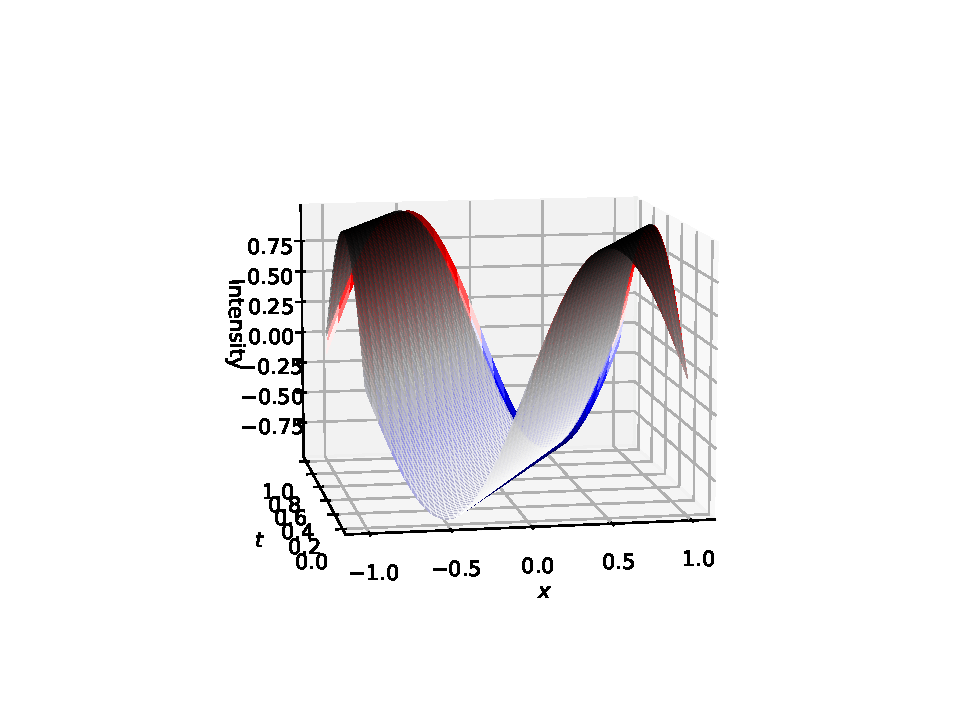
\includegraphics[width=0.85\linewidth]{plots/task4b_numSol.pdf}\label{fig:task4b_numSol}}\hspace{0mm}
\subfloat[Relative error $e^r_{\ell}$]{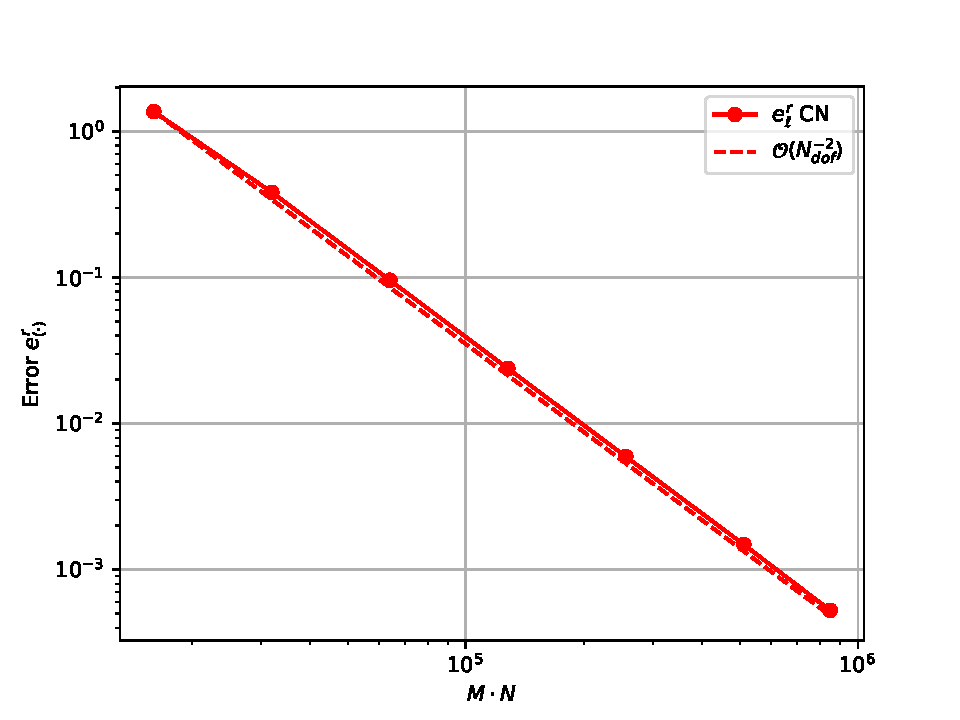
\includegraphics[width=0.85\linewidth]{plots/task4b_error.pdf}\label{fig:task4b_error}}\hspace{0mm}
\caption{Linearized Korteweg-deVries equation on $x \in [-1,1]$ and $t \in [0,1]$, with a periodic boundary condition and initial condition $u(x,0)=\sin{(\pi x)}$. In (a), the analytical solution is shown in grey and the numerical solution is plotted with a \textit{seismic} color map. The numerical solution is calculated using Crank-Nicolson with $M=N=50$. In (b), the relative error $e^r_{\ell}$ at $t=1$ is plotted with the $x$-axis as the number of degrees of freedom. The numerical solution is calculated with Crank-Nicolson where $N=1000$ and $M$ increases exponentially.}
\end{figure}

In order to quantify the convergence of the numerical solution to the analytical solution, the relative error, defined as in equation \eqref{discreteRelativeError}, is calculated. The convergence plot in figure \ref{fig:task4b_error} shows that the discrete $\ell_2$ error goes as $\mathcal{O}(N_{\mathrm{dof}}^{-2})$, as expected, given the truncation error term in \eqref{task4CrankExact}.

\subsubsection{c)}
In this section, a proof of the fact that the continuous $L_2$ norm of the analytical solution in problem \eqref{KdV} is conserved over time, as long as a periodic boundary condition is imposed, will be constructed. The analytical solution can be expressed in a Fourier series on the form

\begin{equation*}
    u(x,t) = \sum_{k \in \mathbb{Z}}\widehat{u}(k,0)\exp{(-i\pi k(1+\pi^2)t + i\pi^3k^3t)}\exp{(i\pi kx)}.
\end{equation*}
Using the notation $u(x,t)^*$ for the complex conjugate of $u(x,t)$, the absolute value of $u(x,t)$ can be expressed with a double summation on the form 

\begin{equation*}
    \begin{split}
        |u(x,t)|^2 &= u(x,t)^* u(x,t) \\ &= \left(\sum_{k \in \mathbb{Z}}\widehat{u}(k,0)^* \mathrm{e}^{i\pi k(1+\pi^2)t - i\pi^3 k^3 t}\mathrm{e}^{-i\pi kx}\right) \left(\sum_{k \in \mathbb{Z}}\widehat{u}(k,0) \mathrm{e}^{-i\pi k(1+\pi^2)t +i\pi^3 k^3t}\mathrm{e}^{i\pi kx}\right) \\ &= \sum_{k\in \mathbb{Z}}\sum_{l \in \mathbb{Z}} \widehat{u}(k,0)^*\widehat{u}(l,0) \mathrm{e}^{i\pi k(1+\pi^2)t-i\pi^3 k^3t}\mathrm{e}^{-i\pi l(1+\pi^2)t+i\pi^3 l^3t }\mathrm{e}^{-i\pi kx}\mathrm{e}^{i\pi lx}.
    \end{split}
\end{equation*}
Integrating over $x \in [-1,1]$ and using the orthogonality of Fourier basis functions, namely that $\int_{-1}^{1} \exp{(-i\pi kx)}\exp{(i\pi lx)} \mathrm{d}x =2\delta_{k,l}$, yields

\begin{equation*}
    \begin{split}
        \int_{-1}^{1} |u(x,t)|^2 \mathrm{d}x &= \sum_{k\in \mathbb{Z}}\sum_{l \in \mathbb{Z}} \widehat{u}(k,0)^*\widehat{u}(l,0) \mathrm{e}^{i\pi k(1+\pi^2)t-i\pi^3 k^3t}\mathrm{e}^{-i\pi l(1+\pi^2)t+i\pi^3 l^3t } \int_{-1}^{1} \mathrm{e}^{-i\pi kx}\mathrm{e}^{i\pi lx} \mathrm{d}x \\ &= 2\sum_{k \in \mathbb{Z}} \widehat{u}(k,0)^*\widehat{u}(k,0) \mathrm{e}^{(i\pi k(1+\pi^2)t-i\pi^3 k^3t)} \mathrm{e}^{-(i\pi k(1+\pi^2)t-i\pi^3 k^3t)} \\ &= 2 \sum_{k \in \mathbb{Z}} \widehat{u}(k,0)^* \widehat{u}(k,0).
    \end{split}
\end{equation*}
In a similar manner, the integral of $|u(x,0)|^2$ can be calculated as 

\begin{equation*}
    \begin{split}
        \int_{-1}^{1} |u(x,0)|^2  &= \sum_{k \in \mathbb{Z}}\sum_{l \in \mathbb{Z}} \widehat{u}(k,0)^*\widehat{u}(l,0) \int_{-1}^{1} \mathrm{e}^{-i\pi kx} \mathrm{e}^{i\pi lx} \mathrm{d}x \\ &= 2\sum_{k \in \mathbb{Z}} \widehat{u}(k,0)^* \widehat{u}(k,0).
    \end{split}
\end{equation*}
Observe that the two integrals are identical to each other. The definition of the $L_2$ norm gives 

\begin{equation*}
\begin{split}
    ||u(x,t)|| &:= \sqrt{\frac{1}{2}\int_{-1}^{1} |u(x,t)|^2\mathrm{d}x} = \sqrt{\frac{1}{2}\int_{-1}^{1} |u(x,0)|^2\mathrm{d}x} \\ &= \sqrt{\sum_{k \in \mathbb{Z}} |\widehat{u}(k,0)|^2}.
\end{split}
\end{equation*}
Hence, the $L_2$ norm is conserved for any time $t > 0$. $\square$

\begin{comment}
One can alternatively show that $\frac{\mathrm{d}}{\mathrm{d}t}|u(x,t)|^2 = 0$. We have 

\begin{equation}
    \frac{\mathrm{d}}{\mathrm{d}t}|u(x,t)|^2 = u_t(x,t)^* u(x, t) + u_t(x, t) u(x, t)^* 
\label{time_der}
\end{equation}

We consider the first term of \eqref{time_der}:

\begin{equation*}
    \begin{split}
        u_t(x,t)^* u(x, t) &= \left(\sum_{k \in \mathbb{Z}}(i\pi k(1 + \pi^2) - i \pi^3 k^3)\widehat{u}(k,t)^* \mathrm{e}^{i\pi k x}\right) \left(\sum_{l \in \mathbb{Z}}\widehat{u}(l,t) \mathrm{e}^{i\pi lx}\right) \\
        &= \sum_{k \in \mathbb{Z}} \sum_{l \in \mathbb{Z}} (i \pi k(1 +\pi^2) - i\pi^3 k^3 ) \mathrm{e}^{i\pi(l - x)} 
    \end{split}
\end{equation*}

\end{comment}

Numerically, the conservation of the $L_2$ norm can be observed by calculating the discrete $\ell_2$ norm and using that as an approximation for the continuous case. By using the discretization method implemented in \textbf{b)}, namely the one based on the Crank-Nicolson method \eqref{task4discCrank}, due to the mentioned stability reasons, the $\ell_2$ norm is calculated as a function of time for two specified initial conditions. The first case is with $u(x,0)=\sin{(\pi x)}$, as in the original problem \eqref{KdV}, and the second case is with $u(x,0)=\sin{(2 \pi x)}$. The plots of the discrete $\ell_2$ norm over time are shown in the figures \ref{fig:task4c_sine} and \ref{fig:task4c_sine_2}. Observe that the $\ell_2$ norm is oscillating around a fixed value and not drifting with time, which is in agreement with the discussion above.

\begin{figure}
\centering
\subfloat[Initial condition $u(x,0)=\sin{(\pi x)}$]{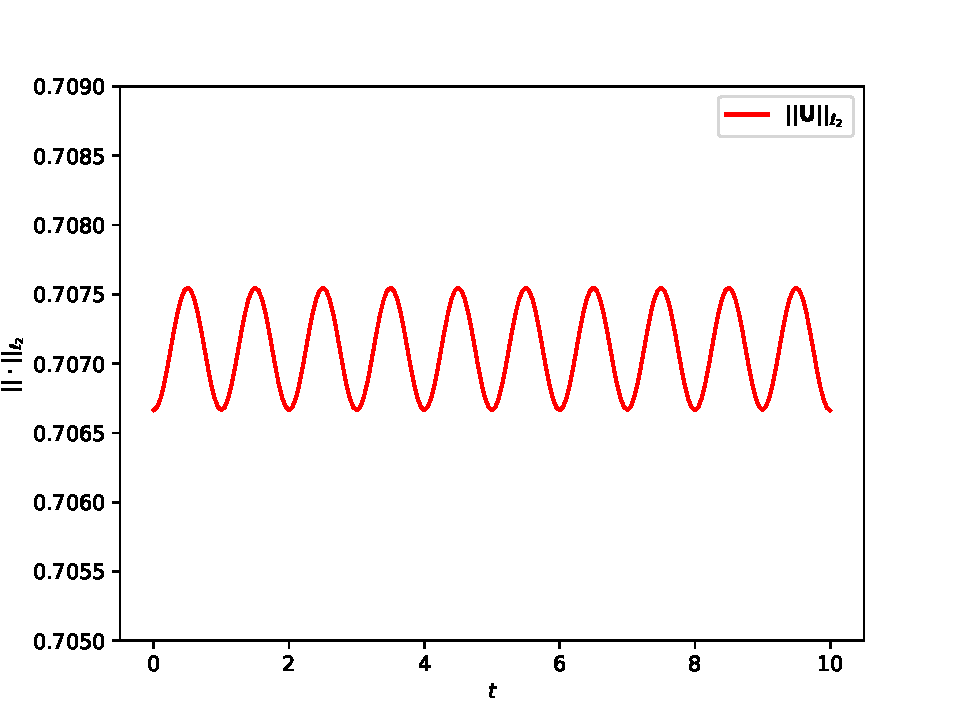
\includegraphics[width=0.85\linewidth]{plots/task4c_sine.pdf}\label{fig:task4c_sine}}\hspace{0mm}
\subfloat[Initial condition $u(x,0)=\sin{(2 \pi x)}$]{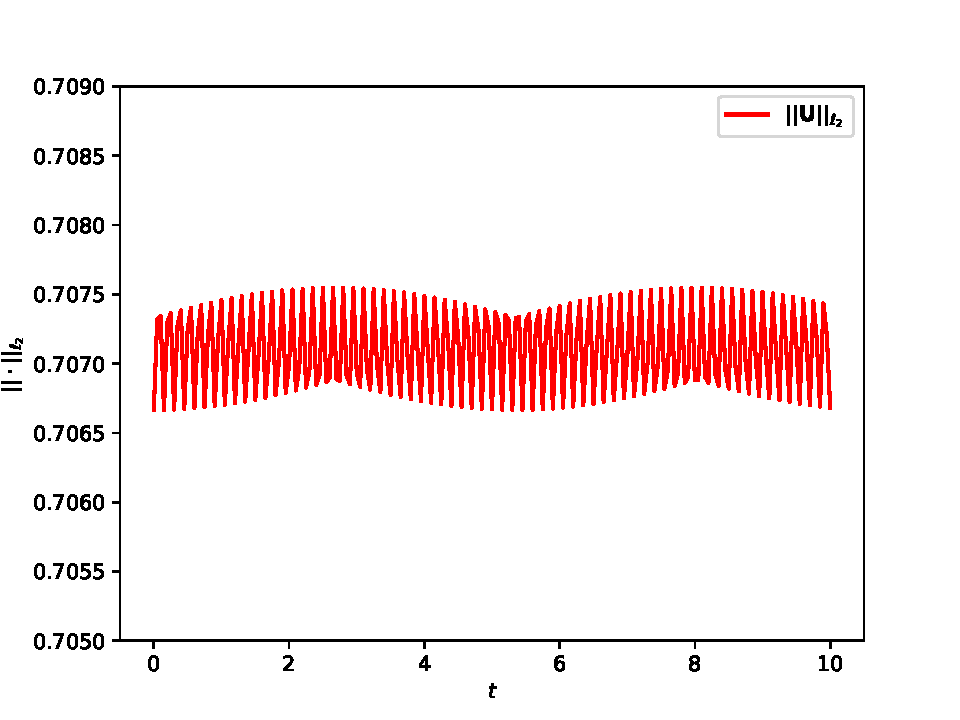
\includegraphics[width=0.85\linewidth]{plots/task4c_sine_2.pdf}\label{fig:task4c_sine_2}}\hspace{0mm}
\caption{Linearized Korteweg-deVries equation on $x \in [-1,1]$ and $t \in [0,10]$, with a periodic boundary condition with period 2. The discrete $\ell_2$ norm of the numerical solution as a function of time, with initial condition $u(x,0)=\sin{(\pi x)}$, is shown in (a) and with initial condition $u(x,0)=\sin{(2 \pi x)}$ in (b). The numerical solution is calculated using the Crank-Nicolson method.}
\end{figure}

\newpage
\ 
\newpage